% !TEX encoding   = UTF8
% !TEX spellcheck = ru_RU
% !TEX root = seminars.tex

%%==================
\chapter{Приложение}
%%==================

%%==========================================
\section{Рисование графиков в \lang{Python}}\label{sect:pyplot}
%%==========================================
Каждый язык имеет свои достоинства и недостатки и, как правило, нацелен на~эффективное решение определённого класса задач. Совместное использование разных языков часто помогает сократить усилия при~разработке программ и повысить гибкость либо удобство создаваемых инструментов. Попробуем продемонстрировать это на~примере визуализации результатов обработки данных лабораторной работы по~физике, которые можно получить методом наименьших квадратов, рассмотренным в~главе~\ref{chap:ide} (также см. упр.~\ref{ex:plot} на~странице~\pageref{ex:plot}).

\begin{figure}[ht]
  {\centering
    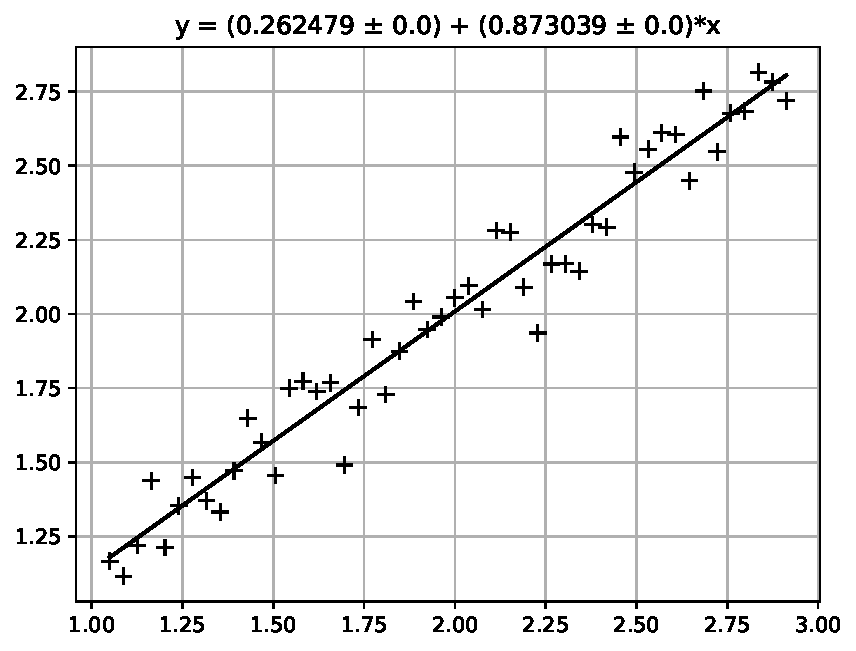
\includegraphics[width=0.6\textwidth]{images/line_approx.pdf}

  }
  \caption{Визуализация при~помощи \name{Matplotlib}}
  \label{fig:pyplot}
\end{figure}

В~языке \lang{C++} нет встроенных графических средств. Для~этого необходимо использовать сторонние библиотеки. Работа с~подобными инструментами не~всегда настолько проста, как хотелось бы. А настройка внешнего вида координатных осей, изображаемых кривых и точек может потребовать перекомпиляции всей программы.

Одним из~действительно удобных для~этого случая решений является написание сценария (\textenglish{script}) на~интерпретируемом языке. \href{\pythonurl}{\lang{Python}} относится к~этому ряду языков и имеет мощную поддержку разнообразных средств практически прямо <<из~коробки>>. Ниже приведён вариант решения нашей задачи с~использованием пакета \href{\matplotliburl}{\name{Matplotlib}}.

\inputminted[linenos, fontsize=\small]{py}{projects/02/plot.py}

Совместить использование разработанных нами отдельных инструментов можно при~помощи командной среды. Для~этого достаточно всего одной строки (см. страницу~\pageref{sect:shell}):
\begin{consolecode}
$ bin/lsm 02/line_approx.txt | xargs python3 02/plot.py
\end{consolecode}

\noindent Результат в~виде графического файла \code{02/line\_approx.pdf}, изображён на~рисунке~\ref{fig:pyplot}.
